\subsection{SDL2 GUI implementation}
\label{sec:sdl2gui}

Since we're using SDL2, we've made an implementation of the UIComponent class
 with the following template arguments:
\begin{itemize}
\item T = SDLRenderer (Our implementation of the SDL2 renderer class)
\item D = sdl\_data (a data structure)
\item R = SDL\_Texture (SDL2's texture structure)
\item S = sdl\_mouse\_event\_data (data used by the mouse callback object)
\end{itemize}

You can also create custom SDL\_UIComponent by inheriting from the 
SDL\_UIComponent class as shown in \cref{fig:sdluicomponent-inherit}. You can 
also use a custom struct that inherits from sdl\_data if your class' 
rendering object uses a different data type. For example, the SDLButton 
rendering object uses a struct that has been derived from the sdl\_data 
struct, which can be seen in \cref{fig:renderobject-inherit}.

\begin{figure}[!htb]
\centering
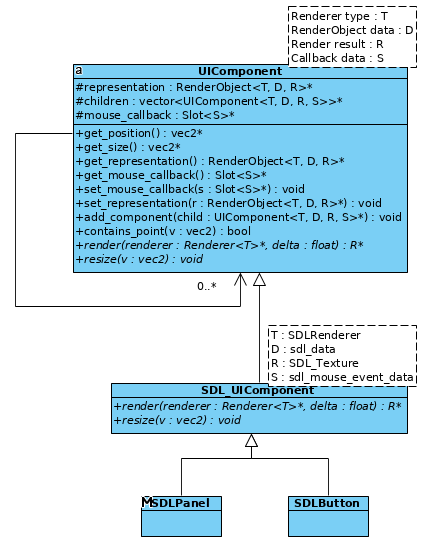
\includegraphics[scale=0.75]{res/ui/sdluicomponent-inherit.png}
\caption{SDL\_UIComponent class inheritance.}\label{fig:sdluicomponent-inherit}
\end{figure}
